\chapter{Introduction}
In this thesis the initial task was to learn how street networks and buildings can be described as grammar for later analysis and regeneration. There exist many different approaches like Shape Grammar \ref{sec:shape_grammar} (building faces generation), L-Systems \ref{sec:L-Systems} (plants growing), Space Syntax \ref{sec:space_syntax} and many others. 

The \textit{Chair of Information Architecture} provided a street generation and analysing tool named CPlan \ref{CPlan}. To become acquainted with the application and to allow using the existing genetic algorithms a tree generating algorithm was developed for this thesis. 

Selecting interesting areas from different cities and recombining them into a new one would allow a fast creation of new cities. To reach this aim many steps are needed. First of all the cities must be separated into reasonable parts based on vertex position or edge length. The approach of this thesis is to use clustering algorithms from the field of machine learning. Then the extracted area should be valued with analysis method to select useful ones.

For this thesis the centroid-based \ref{sec:K-Means} clustering algorithm K-Means was implemented and tested. To correct wrong assignment a shortest path algorithm was used \ref{sec:K-Means_shortest_path} to create connected clusters.

Another approach are the hierarchical clustering algorithms \ref{sec:hierarchicalClustering} were different reduction formula exist. First the Single-Linkage formula was implemented. Unfortunately only one cluster in the center and with many small clusters at the surrounding was created.

Then the reduction formula \acrshort{WPGMA} (\acrlong{WPGMA}) was implemented and tested. The city areas where separated but they vary widely in the size.

To correct this issue the \acrshort{UPGMA} (\acrlong{UPGMA}) reduction formula was used and implemented because every edge counts equal. This approach created better clusters but the cluster sizes were still too different.

Equal clusters sizes then where achieved by modifying the output \ref{sec:outout_modification}. This means instead of splitting the hierarchy as it was created, always the cluster with the most notes was split. As a result the areas where equal sized as preferred in city clustering. The result can be viewed in Figure  \ref{fig:cluster_with_mod_sizes}.

\begin{figure}[ht]
    \centering
    \begin{mdframed}[style=mdthight, userdefinedwidth=0.4\linewidth, align=center]
        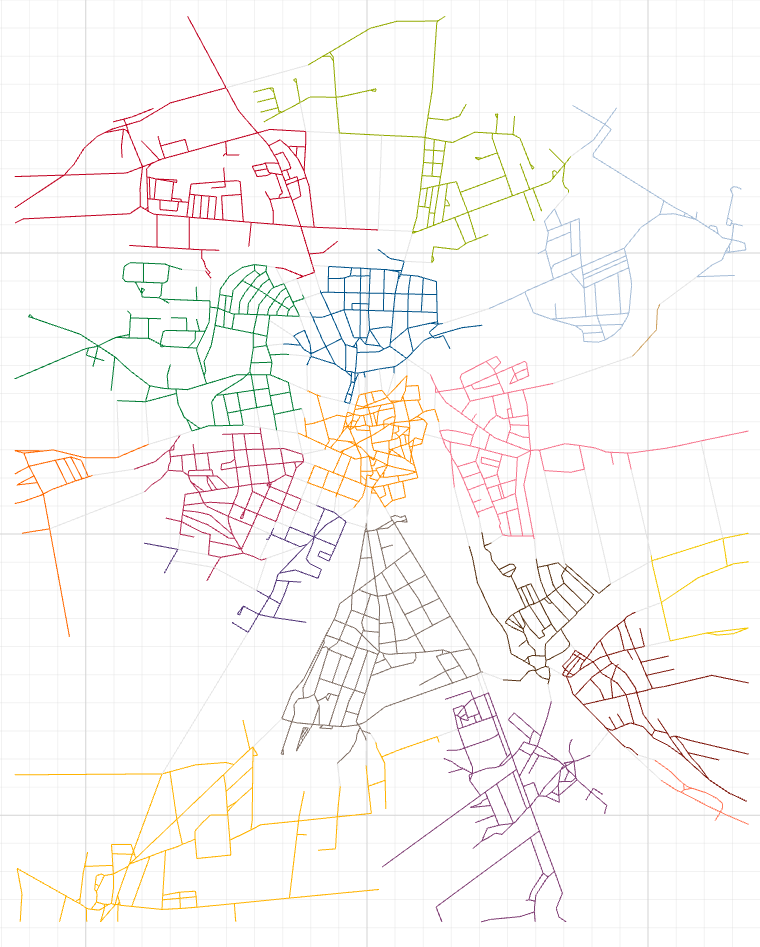
\includegraphics[width=\linewidth]{modified_cluster_size.png}
    \end{mdframed}
    \caption{Clusters with modified size}
    \label{fig:cluster_with_mod_sizes}
\end{figure}

During tests with big cities the hierarchical clustering methods had a hight memory usage. To reduce the memory footprint \ref{sec:memory_usage} optimisations were made and specialized data structures were used.

The created clusters were then measured \ref{sec:measurements} based on the suggestions \ref{sec:clusterRating} provided by the ETH-Zurich and compared \ref{sec:measurements-cluster-analysis}. Additionally the results can now be exported into a JSON-File for further use.

To recombine the separated areas/districts to a new city another project at ETH-Zurich is currently working on a regrow algorithm \ref{sec:future_work}. 